\documentclass[11pt]{article}
\usepackage[sort]{natbib}
\usepackage{bm,amsmath,bbm,amsfonts,nicefrac,latexsym,amsmath,amsfonts,amsbsy,amscd,amsxtra,amsgen,amsopn,bbm,amsthm,amssymb,graphicx, pbox, subcaption}
\usepackage{fancyhdr, tabularx}
\usepackage[margin=1in]{geometry}
\bibliographystyle{abbrvnat}

\title{Using data assimilation to understand the effect of disturbance on a managed woodland}
\author{Ewan Pinnington}

\newtheorem{theorem}{Theorem}[section]
\newtheorem*{defn}{Definition}


\begin{document}

\maketitle


\section*{Abstract}
The response of forests and terrestrial ecosystems to disturbance is an important process in the global carbon cycle in context of a changing climate. Disturbance can take many forms, for example; felling, fire and insect outbreak. In current estimates of the global carbon budget disturbance is one of the least understood components. In this paper we investigate the effect of management practices on the carbon dynamics of a mature temperate woodland. In order to better understand ecosystem response we use the mathematical technique of data assimilation to combine a diverse set of observations with a mathematical model of ecosystem carbon balance. This allows us to combine the uncertainty from observations and prior model predictions to find the best possible estimate to the studied system. We develop new data assimilation techniques allowing for the assimilation of daytime and nighttime net ecosystem exchange observations with a daily time-step model. This allows for the assimilation of much otherwise neglected carbon flux information. These techniques are applicable to other ecosystem models and data assimilation schemes. Previous statistical analyses of eddy covariance data at the study site had suggested that disturbance from thinning resulted in no change to the net carbon uptake of the ecosystem. We show that this is likely due to reduced ecosystem respiration post-disturbance compensating for a reduction in gross primary productivity. Our results support the theory of an upper limit of forest net carbon uptake due to the magnitude of ecosystem respiration scaling with gross primary productivity.  

\section{Introduction}
\subsection{Role of disturbance in the global C cycle}

\subsection{Current theories on terrestrial ecosystem response to disturbance}
Particular focus on effect of management practices on woodland carbon dynamics.


It has been shown that tree roots provide a rhizosphere priming effect, greatly increasing the rate of soil organic carbon decomposition \citep{ELE:ELE1095}.

\citet{ELE:ELE12097} found little change in net CO\(_{2}\) flux following disturbance from mountain pine beetle outbreaks in North America due to concurrent reductions in gross primary productivity and ecosystem respiration.

\subsection{The role of data assimilation for improving estimates to a system}
Combining the errors from model and observations to improve understanding of a systems response to change.

\subsection{What does this paper do?}
Analyse the effect of disturbance from management practices (thinning) for a deciduous managed woodland (Alice Holt) by the combination of a diverse set of observations with a mathematical model of forest carbon balance. Western side of the site thinned in 2014 and the Eastern side left unmanaged. The site has a flux tower positioned on the boundary between managed and unmanaged forest. Eddy covariance observation record was split between two sides using a flux footprint model found in REF. Previous statistical analysis of a management event in 2007 had suggested that there was no change in the Net Ecosystem Exchange (NEE) of CO\(_{2}\) between the managed and unmanaged sides of the forest after thinning. From the years data after the 2014 management event and optimised model in this paper we find evidence to support this and seek an explanation for why the net uptake of carbon remains unchanged even after removing a large proportion of the trees from one side. The data assimilation techniques presented in this paper could be applied for similar analyses at other sites and provide a novel method to help elucidate the reasons behind ecosystem responses.   

\section{Observation and data assimilation methods}

\subsection{Alice Holt research forest} \label{sec:site_description}

Alice Holt Forest is a research forest area managed by the UK Forestry Commission located in Hampshire, SE England. Forest Research has been operating a $\text{CO}_{2}$ flux measurement tower in a portion of the forest, the Straits Inclosure, since 1998 so it is one of the longer forest site $\text{CO}_2$ flux records, globally. The Straits Inclosure is a $90 \text{ha}$ area of managed deciduous broadleaved plantation woodland, presently approximately $80$ years old, on a surface water gley soil. The majority of the canopy trees are oak (\textit{Quercus robur} L.), with an understory of hazel (\textit{Corylus avellana} L.) and hawthorn (\textit{Crataegus monogyna} Jacq.); but there is a small area of conifers (\textit{Pinus nigra} J. F. Arnold) within the tower measurement footprint area in some weather conditions. Further details of the Straits Inclosure site and the measurement procedures are given in \citet{wilkinson2012inter}, together with analysis of stand-scale $30$ minute average net $\text{CO}_{2}$ fluxes (NEE) measured by standard eddy covariance methods from 1998-2011. 

As part of the management regime, the Straits Inclosure is subject to thinning; whereby a proportion of trees are removed from the canopy in order to reduce competition and improve the quality of the final tree crop. At the Straits an intermediate thinning method is used with a portion of both subdominant and dominant trees being removed from the stand \citep{kerr2011thinning}. The whole of the stand was thinned in 1995. Subsequently the Eastern side of the Straits was thinned in 2007 and then the Western side in 2014. The flux tower at the site is situated on the boundary between these two sides, allowing for the use of a footprint model to split the flux record and analyse the effect of this disturbance on carbon fluxes at the site. In \citet{wilkinson2015effects} a statistically analysis of the eddy covariance flux record found that there was no significant effect on the net carbon uptake of the Eastern side after thinning in 2007. In this paper we focus on the effect of disturbance on the Western side after thinning in 2014.   

\subsection{Observations} \label{sec:obs}

In order to assess the effect the 2014 thinning had on the Straits Inclosure an intensive field campaign was undertaken to measure leaf area index and also estimate woody biomass. From the site we also have a long record of flux data as discussed in section~\ref{sec:site_description}.

\subsubsection{Flux tower eddy covariance} \label{sec:eddycov} 

The Straits Inclosure flux tower provides us with half-hourly observations from January 1999 to December 2015, these consist of the NEE fluxes and meteorological driving data of temperatures, irradiance and atmospheric CO\(_{2}\) concentration for use in the DALEC2 model. The NEE data is subject to is subjected to \(u^*\) filtering and quality control procedures as described by \citet{papale2006towards}, but is not gap-filled. This quality controlled half-hourly NEE dataset is then split between observations corresponding to the Western and Eastern sides of the site using a flux-footprint model, see \citet{wilkinson2015effects} for more details.  

For data assimilation NEE observations are usually averaged daily for assimilation with daily time-step ecosystem carbon models. To compute daily NEE observations we take the mean over the 48 measurements made each day, only selecting days where there is no missing data. As we have been strict on the quality control of the flux record and not allowed any gap filling this presents a problem in the number of NEE observations available to us. By splitting the flux record between two sides we retrieve very few total daily observations of NEE for each side. In order to address this we instead compute day and nighttime NEE fluxes (NEE\(_{day}\) and NEE\(_{night}\) respectively) for use in data assimilation. To compute daytime or nighttime NEE observations we take the mean over the half-hourly day or nighttime (calculated using a solar model) measurements, again only taking periods where there are no gaps in the data so that we are only considering true observations. This provides us with many more observations for assimilation after data processing, as seen in table~\ref{table:nee_obs}, as we are averaging over shorter time periods so have a smaller probability of gaps and erroneous data. We see that we have many more daytime NEE observations than nighttime, as we tend to have much more turbulent air mixing in daylight hours. In section~\ref{sec:da} we give details of how we relate these twice daily observations of NEE to a daily time-step model.     

\begin{table}[ht] 
\begin{center}
	\begin{tabular}{| l | l | l | l | l |}
	\hline
	Sector & NEE & NEE\(_{day}\) & NEE\(_{night}\)  \\ \hline
	East & 3 & 57 & 2 \\ \hline
	West & 9 & 50 & 18 \\ \hline
	\end{tabular}
	\caption{Number of observations of NEE, NEE\(_{day}\) and NEE\(_{night}\) for East and West sides of the Straits Inclosure for the year 2015.}
	\label{table:nee_obs}
\end{center} 
\end{table}

In \citet{Richardson200838} the measurement error in observations of daily NEE is found to be between $0.2$ to $0.8~\text{g C m}^{-2} \text{day}^{-1}$.  \citet{Richardson200838} also shows that flux errors are heteroscedastic. In order to account for this we assume a standard deviation of $0.7 + 0.05|\text{NEE}_{\text{day}}^{i}|~\text{g C m}^{-2} \text{day}^{-1}$ in our observations of daytime NEE, where \(|\text{NEE}_{\text{day}}^{i}|\) is the magnitude of the daytime NEE observation. We found this standard deviation gave the best weighting to the observations in the assimilation algorithm while also making some attempt to account for the heteroscedastic nature of the flux errors. \citet{raupach2005model} comment that daytime NEE errors are between 20-50\(\%\) of the observed value while nighttime measurements are much more uncertain. For this reason we specify the standard deviations of nighttime NEE observations as $1.2 + 0.15|\text{NEE}_{\text{night}}^{i}|~\text{g C m}^{-2} \text{day}^{-1}$. We also include correlations in time between the errors in our observations of NEE, as discussed in \citet{Pinnington2016299}.

\subsubsection{Leaf area index}

As part of the work undertaken for this paper; to assess the impact of the 2014 thinning, three transects were established in the Straits Inclosure for intensive sampling during 2015. A total of 435 sampling points were marked at 10m apart using a GPS unit and fluorescent tree spray paint. Measurements of peak LAI (July 2015 - September 2015) were made using both a ceptometer and hemispherical photography. The transects were walked twice with the ceptometer sampling every 10m, giving 870 readings in total. Hemispherical photographs were taken every 50m as shown in Figure~\ref{fig:hemi_lai} giving 89 photographs in total. 

The ceptometer is used with an additional Photosynthetically Active Radiation (PAR) sensor. We measure below canopy PAR using the ceptometer while logging above canopy PAR using a data logger and PAR sensor positioned outside the canopy. We can then estimate LAI using the above and below canopy readings and a set of equations relying on some assumptions \citep{fassnacht1994comparison}.
For the hemispherical photographs we use the HemiView software \citep{rich1999hemiview} which can calculate the proportion of visible sky as a function of sky direction (gap fraction) this can then be used to calculate LAI  \citep{Jonckheere2004}.

Six litter traps were also established at points along the transects allowing for comparison with the other methods. These were sampled throughout the season in 2015. We found the litter trap derived LAI was always greater than LAI estimates derived from optical methods, as expected \citep{breda2003ground}. From the sampling of the litter traps we also have estimates to leaf mass per area for use in data assimilation. As the 6 litter traps are not enough to describe the LAI for the research site \citep{kimmins1973some}, we used estimates from the ceptometer and hemispherical photographs for data assimilation. We take the weighted average of the hemispherical photograph and ceptometer estimated LAI to find an LAI of 4.42 with a standard error of 0.07 for the Eastern unthinned section of forest and an LAI of 3.06 with a standard error of 0.07 for the Western thinned section of forest. From our litter trap observations we find a leaf mass per area of 29 g C m\(^{-2}\) for both sides of the forest.


\begin{figure}[ht]
    \centering
    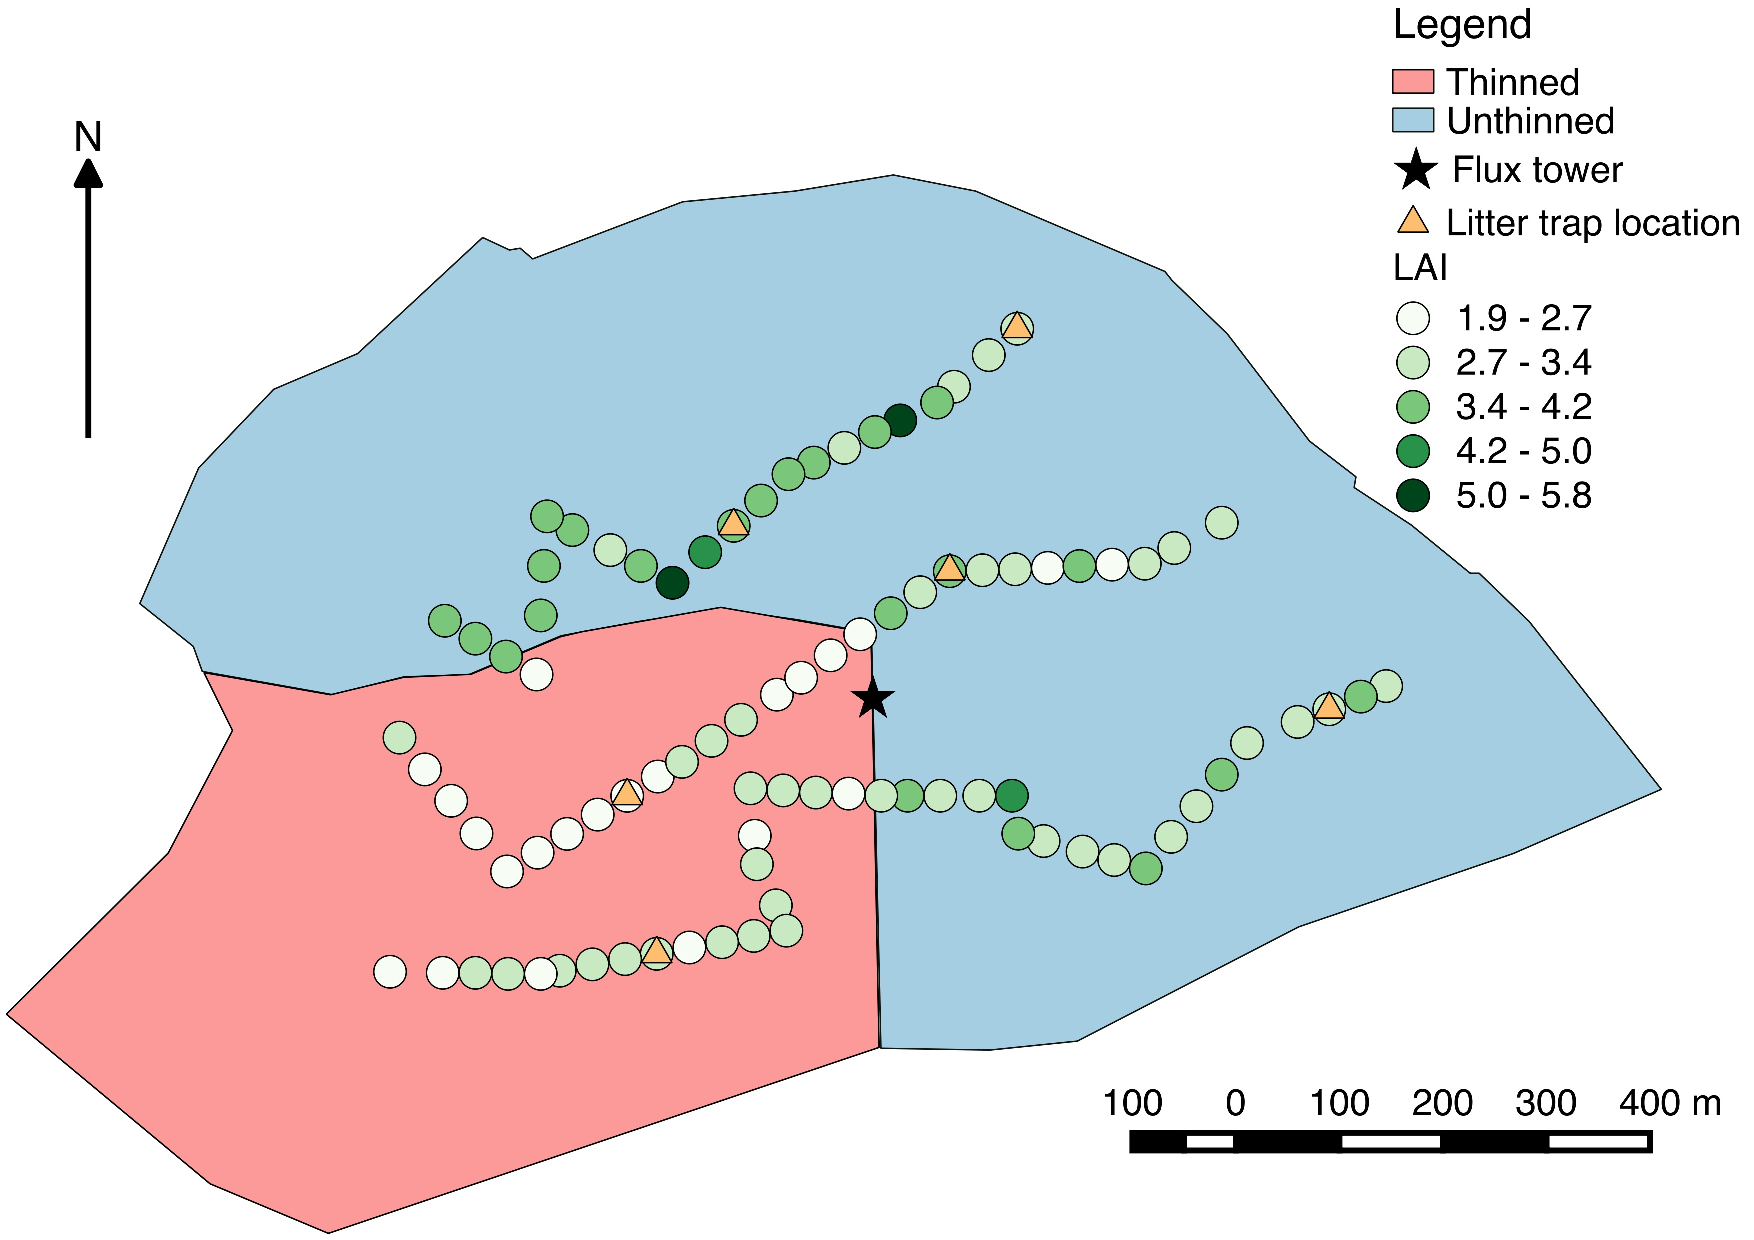
\includegraphics[width=0.5\textwidth]{thinned.pdf}
    \caption{Hemispherical photograph derived LAI for the Straits Inclosure at 50m intervals along three transects.} \label{fig:hemi_lai}
\end{figure}

\subsubsection{Woody biomass}  
The method of Point-Centred Quarters (PCQ) was used to conduct a biomass survey as specified in \citet{dahdouh2006empirical}. 114 points were sampled along the three transects measuring the Diameter at Breast Height (DBH) and the density of trees. We then used allometric relationships between DBH and total above ground biomass and coarse root biomass, found in work carried out by Forest Research and in \citet{mckay2003woodfuel}, to find an estimate to total woody and coarse root carbon. We can see these observations in table~\ref{table:cwoo_obs}, we have made the assumption that 50\% of dry plant mass is carbon.

Forest Research also carry out their own mensuration studies at the site. One such study was carried out of the Western side after the thinning at a similar time to our own PCQ measurements and found a tree density of 225 ha\(^{-1}\) and an average DBH of 32 cm, which are in close agreement to our own estimates in table~\ref{table:cwoo_obs}. This gives us confidence that past measurements before the thinning will also be representative of the methods we have used. From 2009 measurements from Forest Research found the Western side to have a tree density of 418 ha\(^{-1}\) and an average DBH of 27.73 cm. This suggests that approximately 46\% of trees have been removed during thinning. From these estimates we can also see the effect thinning has on the type of trees found at the site. The amount of trees per hectare has dropped dramatically after thinning but the mean DBH has increased, indicating that smaller subdominant trees have been removed. The mean DBH on the Eastern side is greater still, indicating that the thinning that took place in 2007 of the Eastern side has allowed the dominant trees to grow as a result of reduced competition.

\begin{table}[ht] 
\begin{center}
	\begin{tabularx}{\textwidth}{| l | l | l | X |}
	\hline
	Sector & Tree density (ha\(^{-1}\)) & mean DBH (cm) & Estimated Woody biomass and coarse root carbon (g C m\(^{-2}\)) \\ \hline
	East & 272 & 34.12 & 13130 \\ \hline
	West & 225 & 32.85 & 9908 \\ \hline
	\end{tabularx}
	\caption{Point-centred quarter method observations for 2015.}
	\label{table:cwoo_obs}
\end{center} 
\end{table}

\subsection{Model and data assimilation}
\subsubsection{DALEC2 ecosystem carbon model} \label{sec:dalec2}

The DALEC2 model is a simple process-based model describing the carbon dynamics of a forest ecosystem \citep{Bloom2015}. The model is constructed of six carbon pools (labile ($C_{lab}$), foliage ($C_f$), fine roots ($C_r$), woody stems and coarse roots ($C_w$), fresh leaf and fine root litter ($C_l$) and soil organic matter and coarse woody debris ($C_s$)) linked via fluxes. The aggregated canopy model (ACM) \citep{williams1997predicting} is used to calculate daily gross primary production ($GPP$) of the forest, taking meteorological driving data and the modelled leaf area index (a function of $C_f$) as arguments. Figure~\ref{fig:DALEC_mod} shows a schematic of how the carbon pools are linked in DALEC2, full model equations can be found in the appendix, section \ref{sec:dalec_eqns}.   

\begin{figure}[ht]
    \centering
    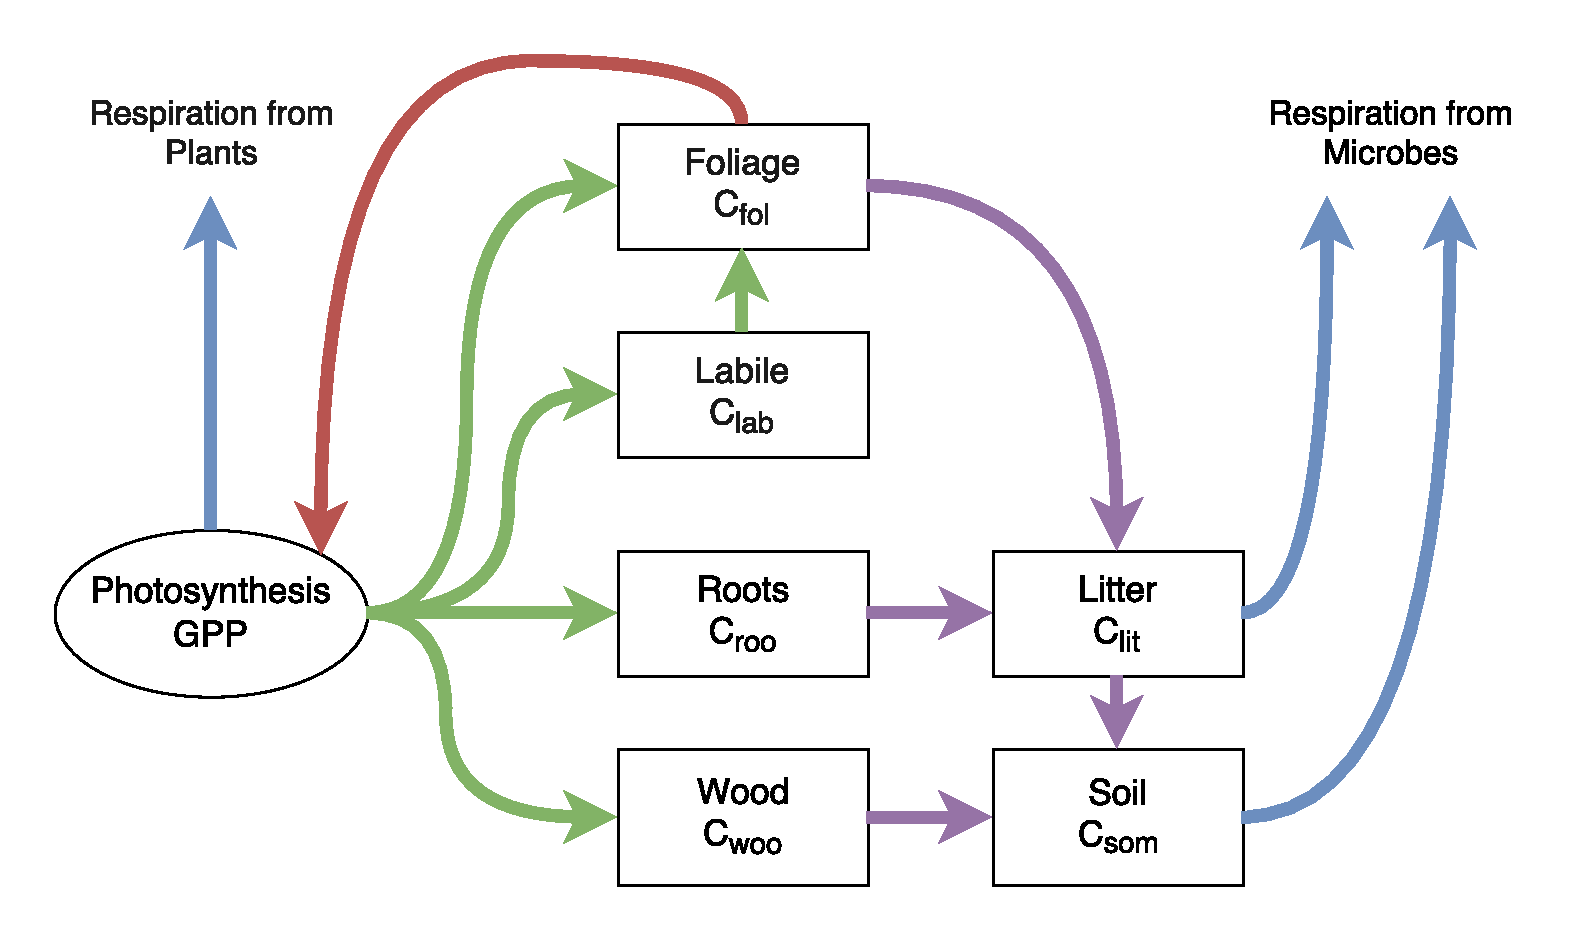
\includegraphics[width=0.5\textwidth]{dalec2diag.pdf}
    \caption{Representation of the fluxes in the DALEC2 carbon balance model. Green arrows represent C allocation, purple arrows represent litter fall and decomposition fluxes, blue arrows represent respiration fluxes and the red arrow represents the influence of leaf area index in the $GPP$ function.} \label{fig:DALEC_mod}
\end{figure}

\subsubsection{Data assimilation} \label{sec:da}

We implement Four-Dimensional Variation data assimilation (4D-Var) with the DALEC2 model for joint parameter and state estimation. In 4D-Var we aim to find the parameter and initial state values such that the model trajectory best fits the data over some time window, given some prior information about the system. This prior information takes the form of an initial estimate to the parameter and state variables of the model, $\textbf{x}^{b}$, valid at the initial time. This prior is assumed to have unbiased, Gaussian errors with known covariance matrix $\textbf{B}$. Adding the prior term ensures that our problem is well posed and that we can find a locally unique solution \citep{Tremolet2006}. The prior used in this paper is derived from the assimilation of eddy covariance data from previous years and can be found in table~\ref{table:xbvars}. In 4D-Var we aim to find the parameter and initial state values that minimises the weighted least squares distance to the prior while minimising the weighted least squares distance of the model trajectory to the observations over the time window $t_{0}, \dots, t_{N}$ \citep{lawless2013}. We do this by finding the state $\textbf{x}^{a}_{0}$ at time $t_{0}$ that minimises the cost function

\begin{equation}
J(\textbf{x}_0) = \frac{1}{2}(\textbf{x}_0-\textbf{x}^b)^{T}\textbf{B}^{-1}(\textbf{x}_0-\textbf{x}^b)+\frac{1}{2}\sum_{i=0}^{N}(\textbf{y}_i-\textbf{h}_i(\textbf{x}_i))^{T}\textbf{R}_{i}^{-1}(\textbf{y}_i-\textbf{h}_i(\textbf{x}_i)),
\end{equation}
where $\textbf{x}_{0}$ is the vector of parameter and initial state values to be optimised, $\textbf{h}_{i}$ is the observation operator mapping the parameters and state to the observations $\textbf{y}_{i}$ and $\textbf{R}_{i}$ is the observation error covariance matrix. Further details of the implemented data assimilation scheme and specification of prior and observational errors can be found in \citet{Pinnington2016299}. 

In this paper we assimilate day and nighttime NEE in order to increase the number of observations available to us and also better partition our modelled estimate of GPP and total ecosystem respiration, as discussed in section~\ref{sec:eddycov}. As the DALEC2 model runs at a daily time step this requires us to relate the daily parameter and state values from the model to the twice-daily observations of NEE. We do this by writing two new observation operators, one relating the model state and parameters to daytime NEE and the other to nighttime NEE. The NEE of CO\(_{2}\) at any given time is the difference between GPP and ecosystem respiration. For an observation of total daily NEE on day \(i\) we have,
\begin{equation}
NEE^{i}=-GPP^{i}(C_{fol}^{i}, \Psi) +f_{auto}GPP^{i}(C_{fol}^{i}, \Psi) + \theta_{lit}C_{lit}^i e^{\Theta T^{i}} + \theta_{som}C_{som}^i e^{\Theta T^{i}}, \label{eqn: D1_nee}
\end{equation}
where all terms have the same meaning as described in section~\ref{sec:dalec_eqns}, with term one being gross primary productivity, term two corresponding to autotrophic respiration and term three and four corresponding to heterotrophic respiration. For total daytime NEE we have,
\begin{equation}
NEE_{day}^{i} = -GPP^{i}(C_{fol}^{i}, \Psi) + \delta_{day}f_{auto}GPP^{i}(C_{fol}^{i}, \Psi) + \delta_{day}\theta_{lit}C_{lit}^i e^{\Theta T_{day}^{i}} + \delta_{day}\theta_{som}C_{som}^i e^{\Theta T_{day}^{i}} \label{eqn: D1_nee_day}
\end{equation}
where \(\delta_{day}\) is the day length, expressed as \(\frac{\text{number of daylight hours}}{24}\), and \(T_{day}^{i}\) is the mean daytime temperature. Here we still have the same term for GPP as in equation~\eqref{eqn: D1_nee} as all photosynthesis occurs during daylight hours, the respirations are then scaled by the length of daylight hours. For nighttime NEE we have,
\begin{equation}
NEE_{night}^{i} =  \delta_{night}f_{auto}GPP^{i}(C_{fol}^{i}, \Psi) + \delta_{night}\theta_{lit}C_{lit}^i e^{\Theta T_{night}^{i}} + \delta_{night}\theta_{som}C_{som}^i e^{\Theta T_{night}^{i}} \label{eqn: D1_nee_night}
\end{equation}
where \(\delta_{night}\) is the night length, expressed as \(\frac{\text{number of night hours}}{24}\), and \(T_{night}^{i}\) is the mean nighttime temperature. Here we no long have a term for GPP as no GPP will occur during the night, the respirations are again scaled by night length as in equation~\eqref{eqn: D1_nee_day}. Day length and night length are calculated using a solar model here, but could also be estimated using the record of incident solar radiation from the flux tower. These new observation operators allow for assimilation of day/nighttime NEE without the need for model development and can be applied to other ecosystem models to allow for the assimilation of finer temporal resolution eddy covariance data and possible improvements to the partitioning of photosynthesis and ecosystem respiration. From section~\ref{sec:results} we can see that these modified observation operators allow our model to predict both daytime and nighttime NEE accurately.

%Cite MacBean?? for correlations?

\subsection{Experimental setup}
%Assimilation of 2015 years data post disturbance for the optimisation of two parameter sets, one corresponding to the unmanaged East and the other set to the managed West.

%In this paper we have split the flux tower eddy covariance record using a footprint model. This means we have observations of NEE for both the West and East sides of the forest stand. By combining these two distinct sets of observations with our prior model using 4D-Var data assimilation allows us to retrieve two unique sets of parameter and initial state values, .

Using the prior model estimate specified in table~\ref{table:xbvars} we run two data assimilation experiments for the years window of 2015. In the first experiment we assimilated all data available (as specified in section~\ref{sec:obs}) for the unthinned Eastern section of forest. In the second experiment we assimilate all data available for the thinned Western section of forest. Combining these two distinct sets of observations with our prior model using 4D-Var data assimilation allows us to retrieve two unique sets of parameter and initial state values corresponding to the thinned and unthinned sections of the site. This allows us to judge the effect the thinning in 2014 had on the carbon dynamics of the forest in 2015. We do this by analysing the optimised parameter and initial state values for the thinned and unthinned sections of the forest and also considering the model predictions of different variables for each side post-disturbance. 

\section{Results} \label{sec:results}
Show plots of East and West after assimilation and the change in optimised parameters. Confident in results as we know that even assimilating a single year of data we can accurately describe the carbon dynamics of the site for a long time period (15 years) into the future from Pinnington et al 2016.

\begin{figure}[ht]
    \centering
    \begin{subfigure}[b]{0.49\textwidth}
        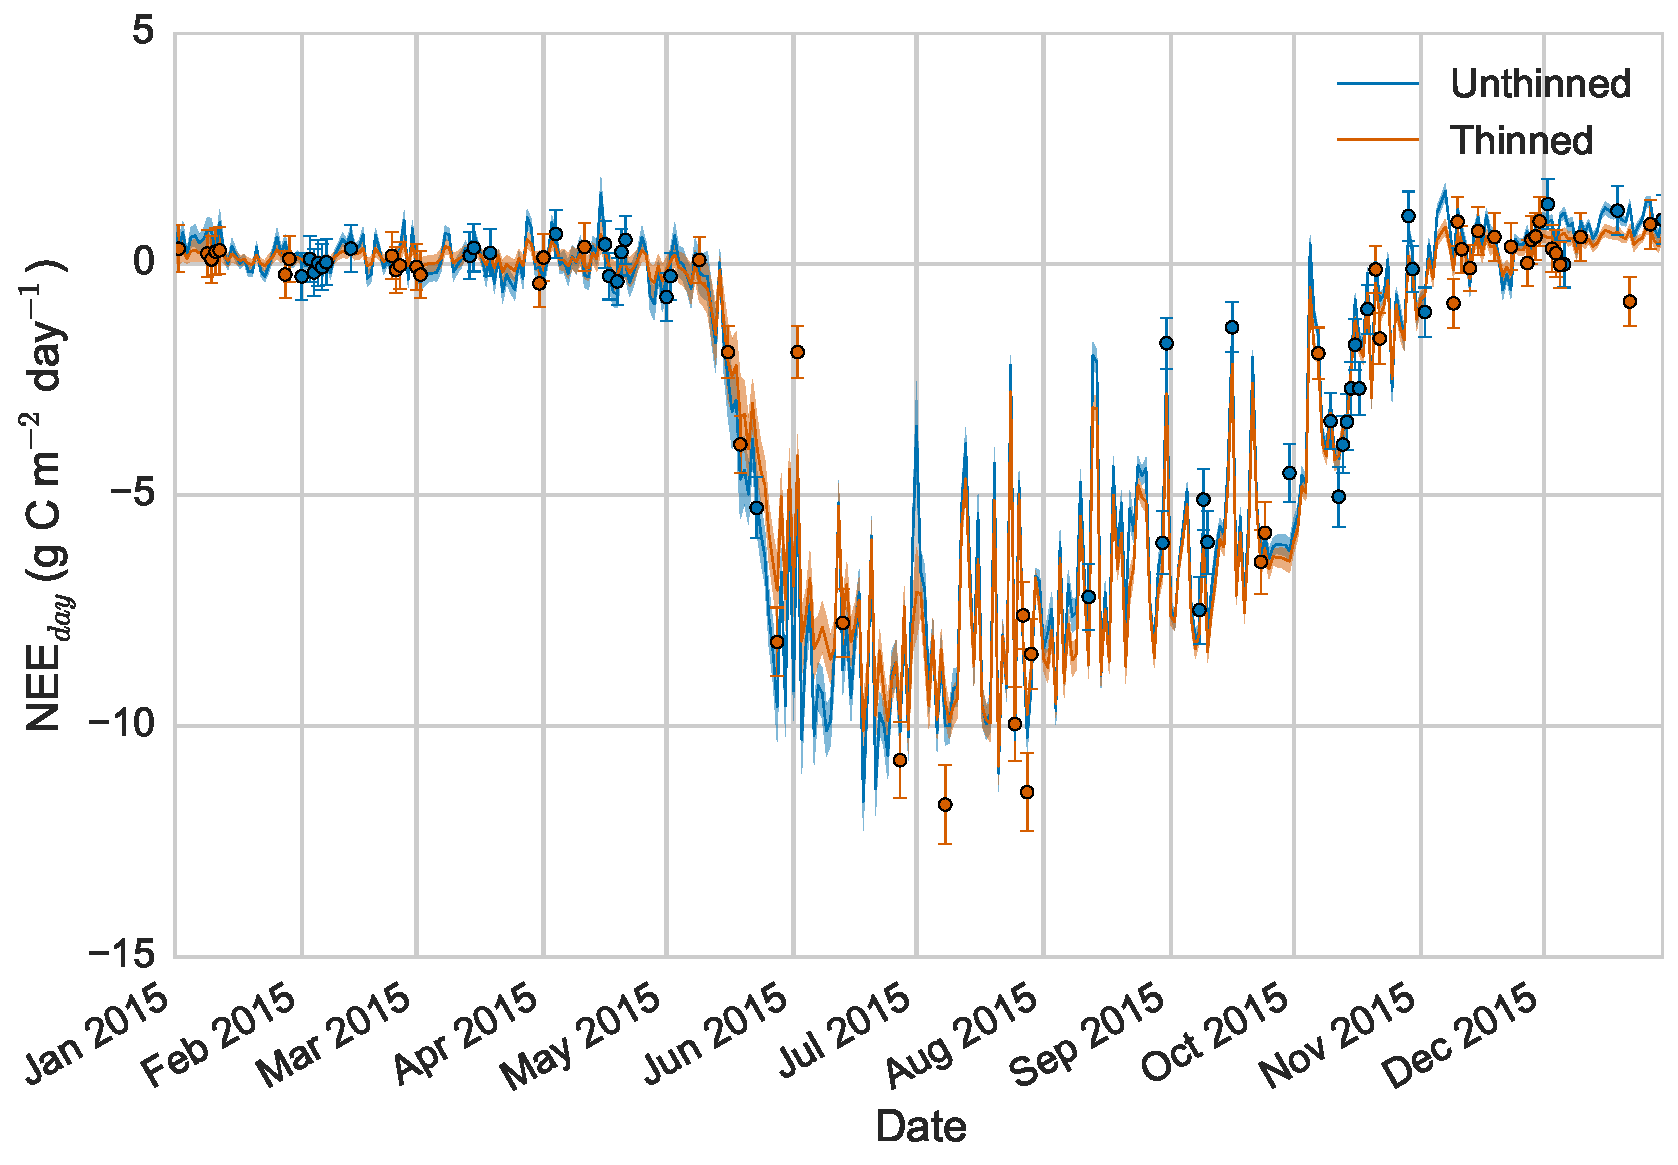
\includegraphics[width=\textwidth]{nee_day.pdf}
        \caption{NEE\(_{day}\)}
        \label{fig:nee_day}
    \end{subfigure}
    \begin{subfigure}[b]{0.49\textwidth}
        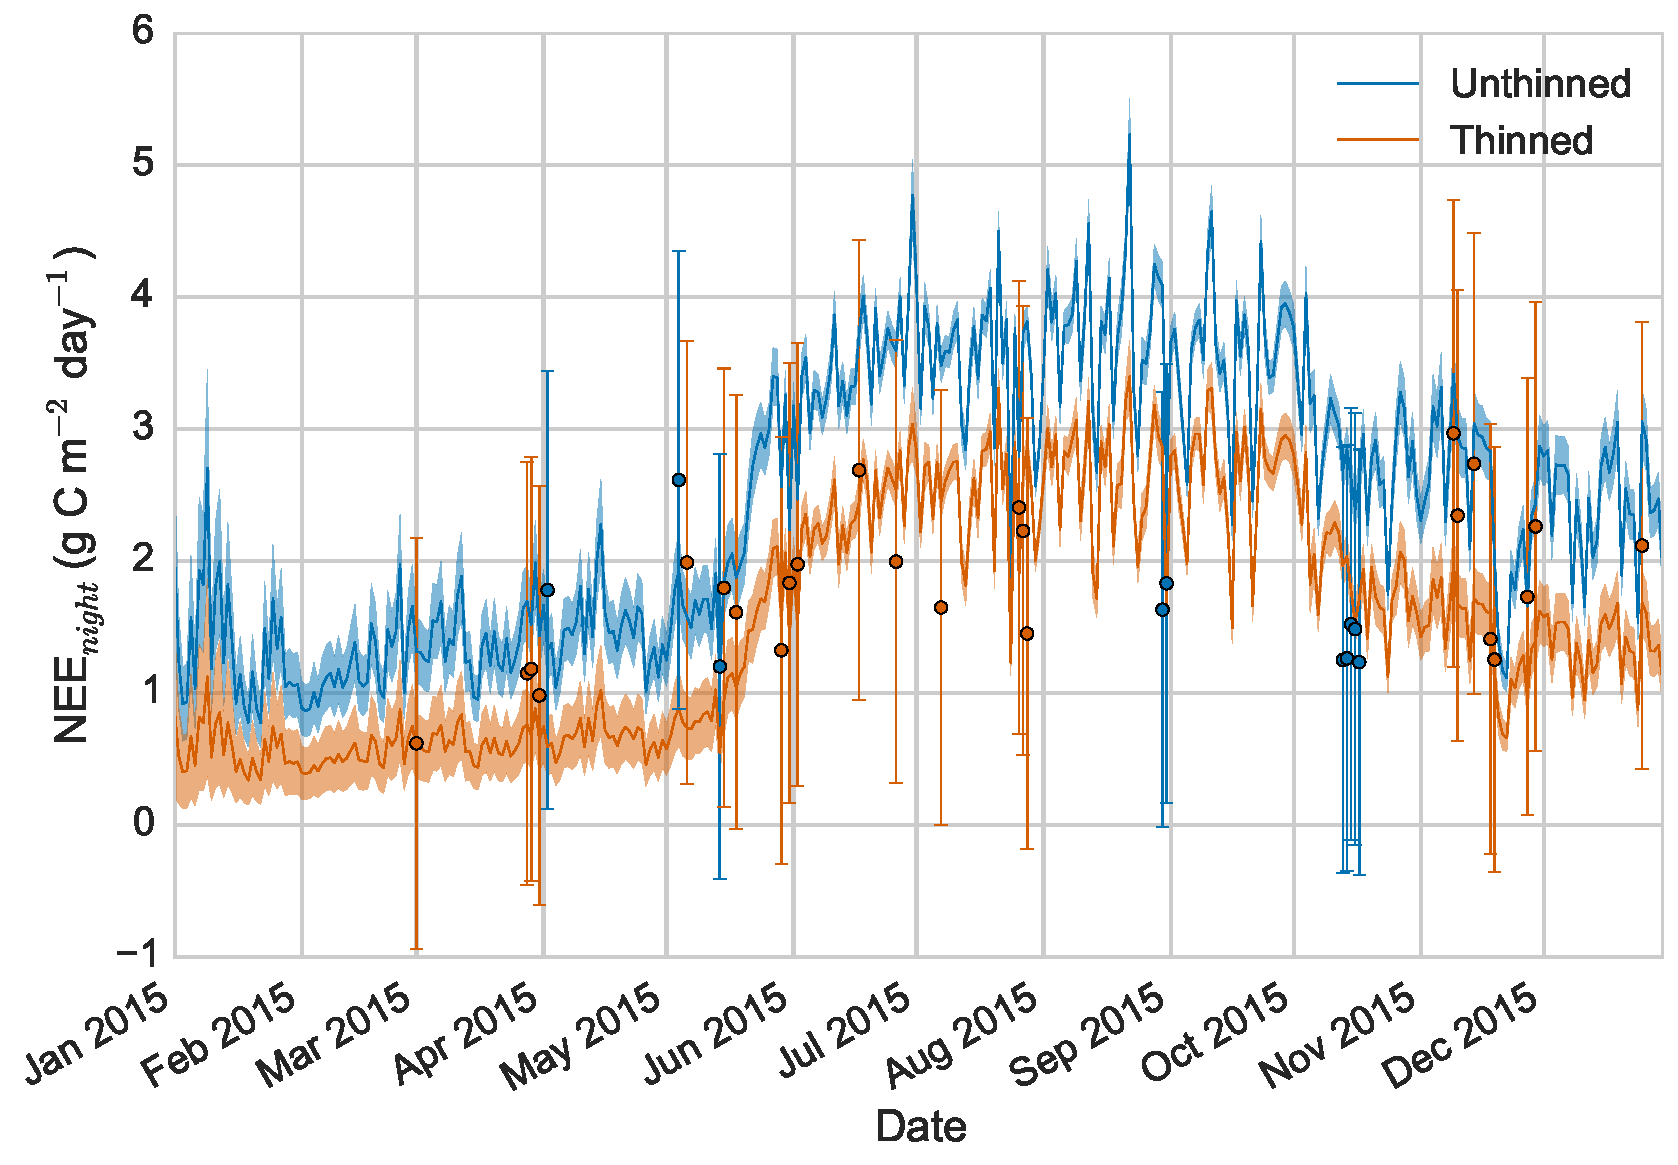
\includegraphics[width=\textwidth]{nee_night.pdf}
        \caption{NEE\(_{night}\)}
        \label{fig:nee_night}
    \end{subfigure}
    \begin{subfigure}[b]{0.49\textwidth}
        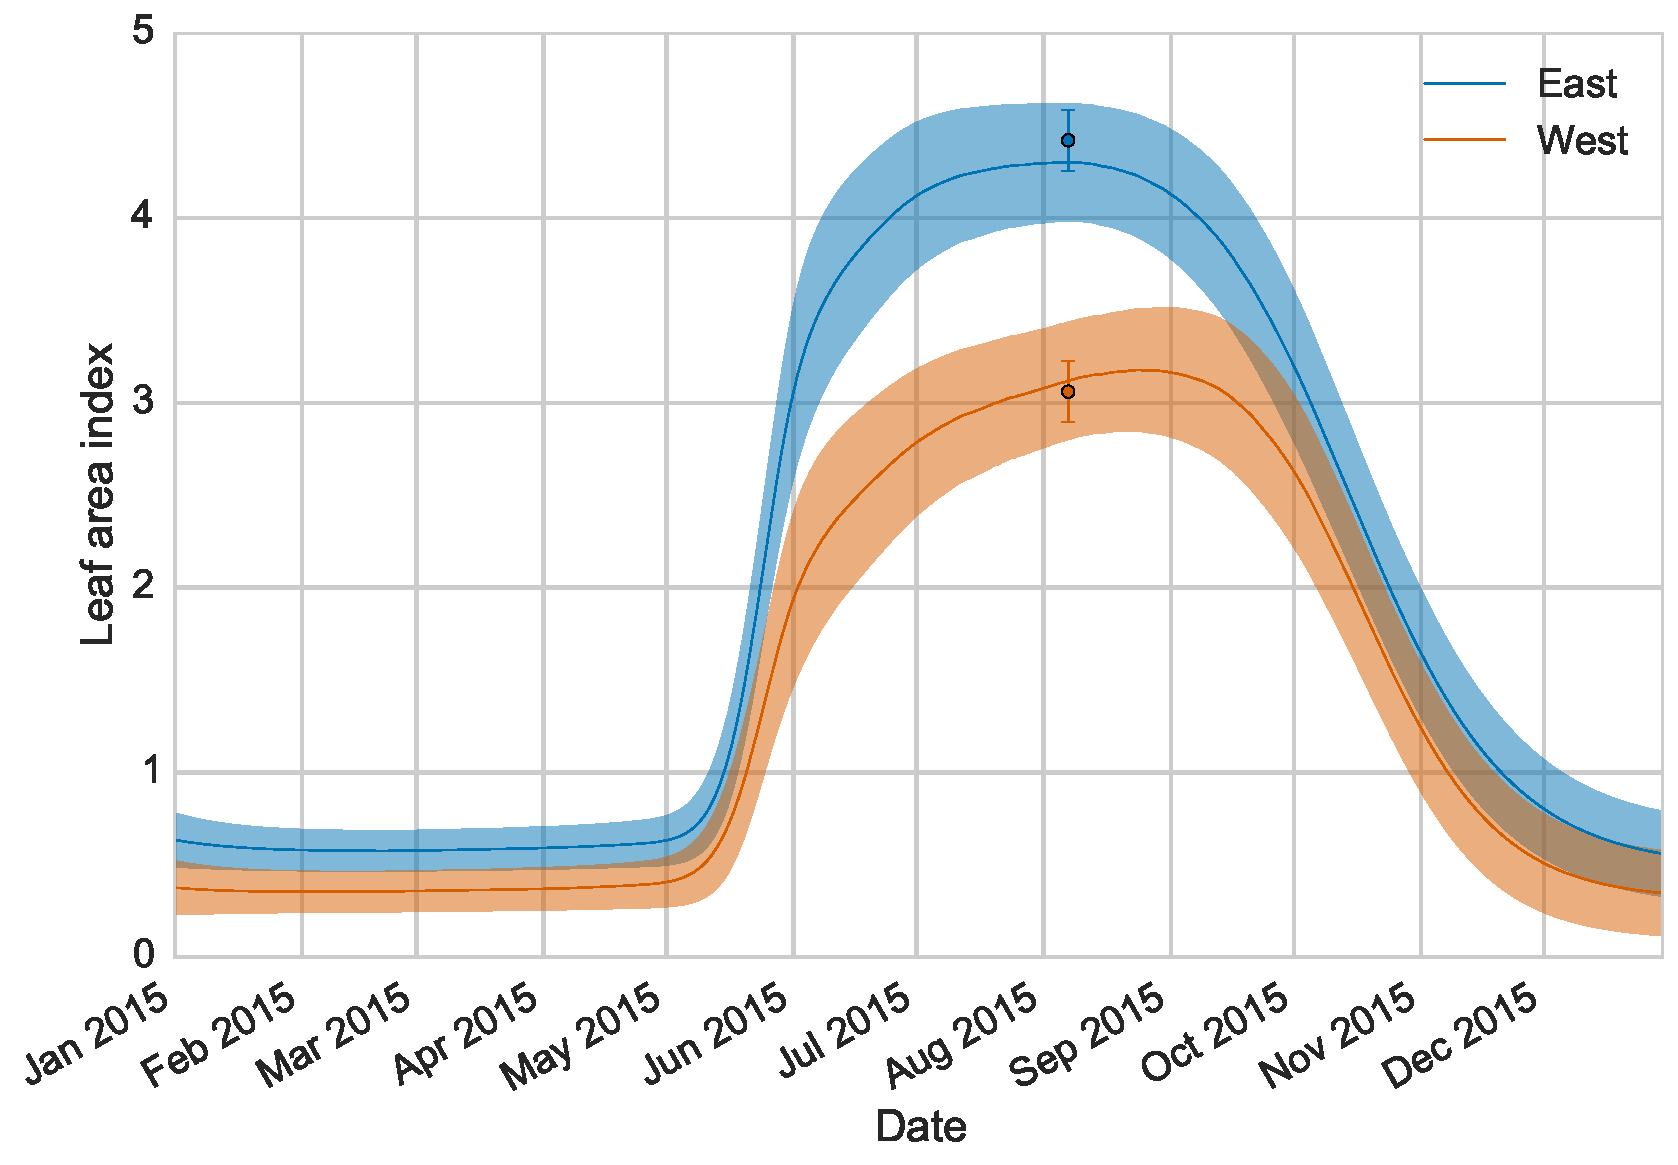
\includegraphics[width=\textwidth]{lai.pdf}
        \caption{Leaf area index}
        \label{fig:lai}
    \end{subfigure}
    \begin{subfigure}[b]{0.49\textwidth}
        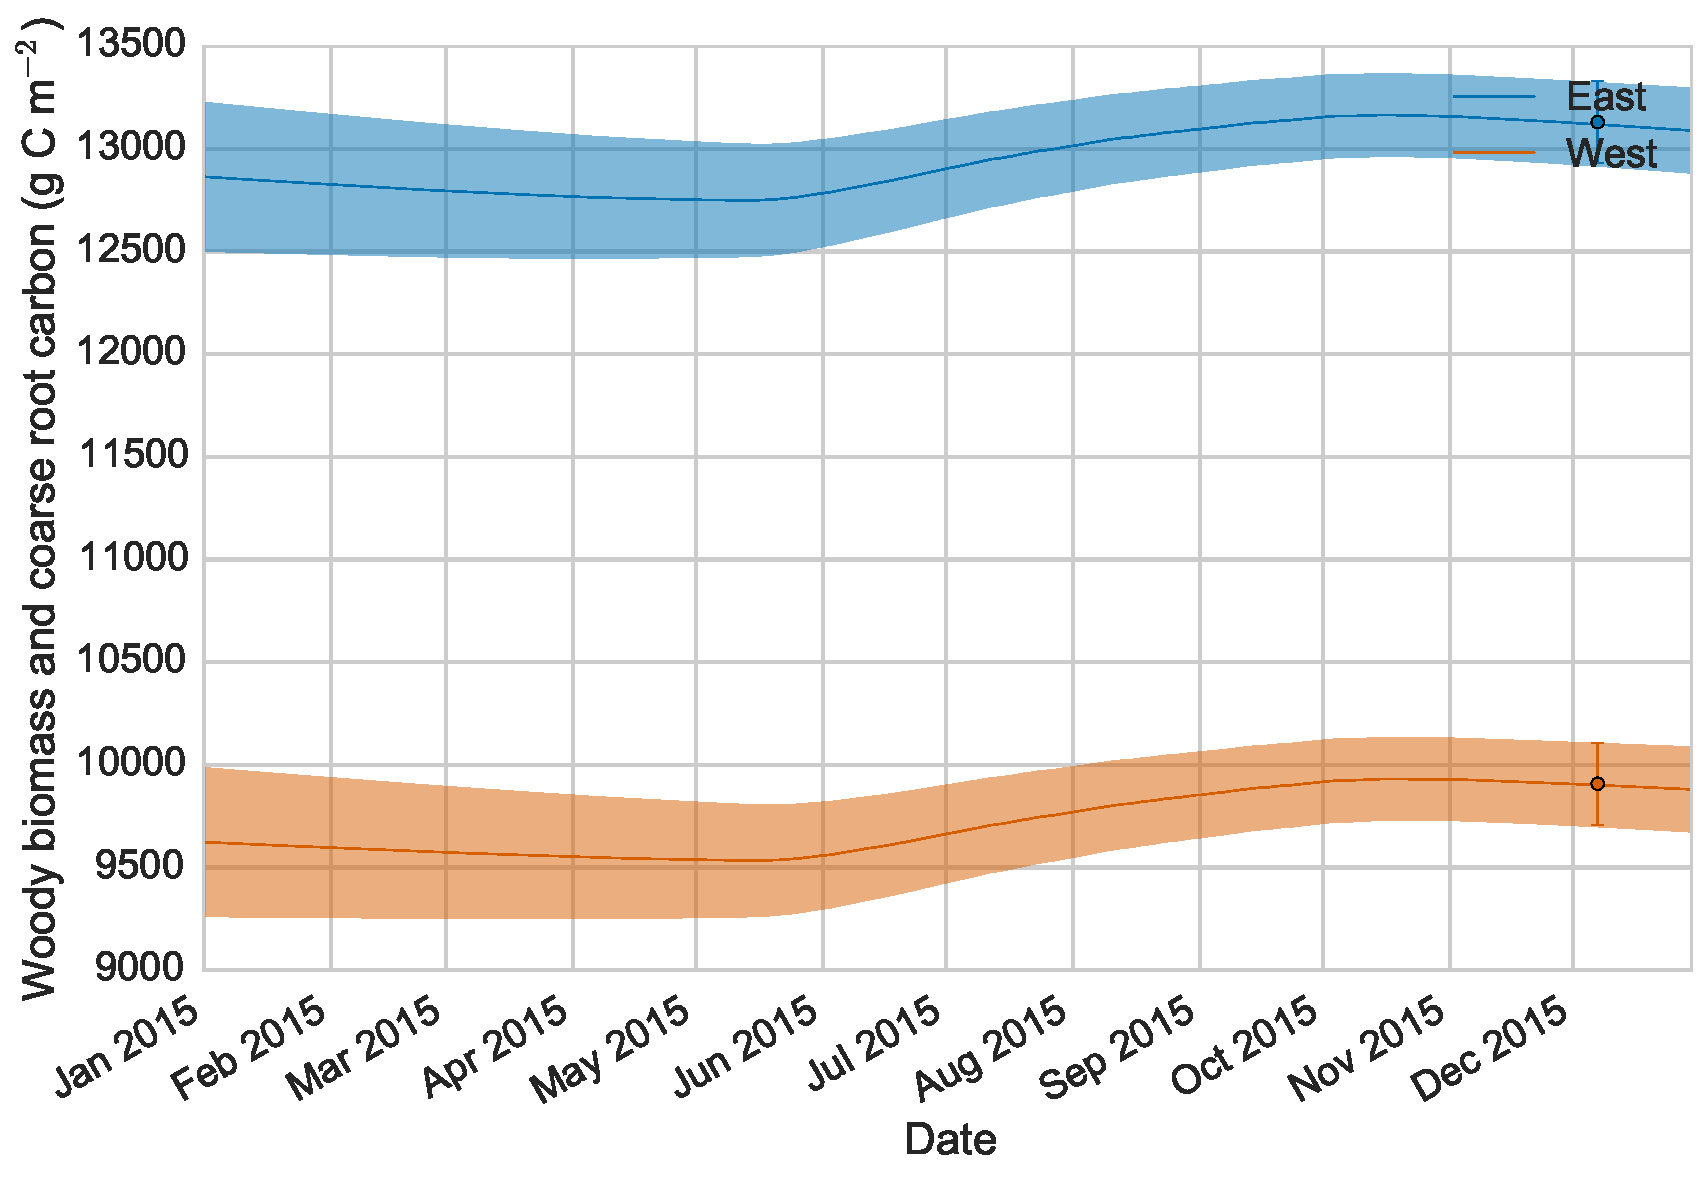
\includegraphics[width=\textwidth]{c_woo.pdf}
        \caption{C\(_{woo}\)}
        \label{fig:c_woo}
    \end{subfigure}
    \caption{2015 East and West observations and model trajectories after assimilation. Blue line: model trajectory after assimilation of East data, blue shading: error in model after assimilation (\(\pm\) 1 standard deviation), blue dots: East observations with error bars, orange line: model trajectory after assimilation of West data, orange shading: error in model after assimilation (\(\pm\) 1 standard deviation), orange dots: West observations with error bars.} \label{fig:nee_day}
\end{figure}

\begin{figure}[ht]
    \centering
    \begin{subfigure}[b]{0.49\textwidth}
        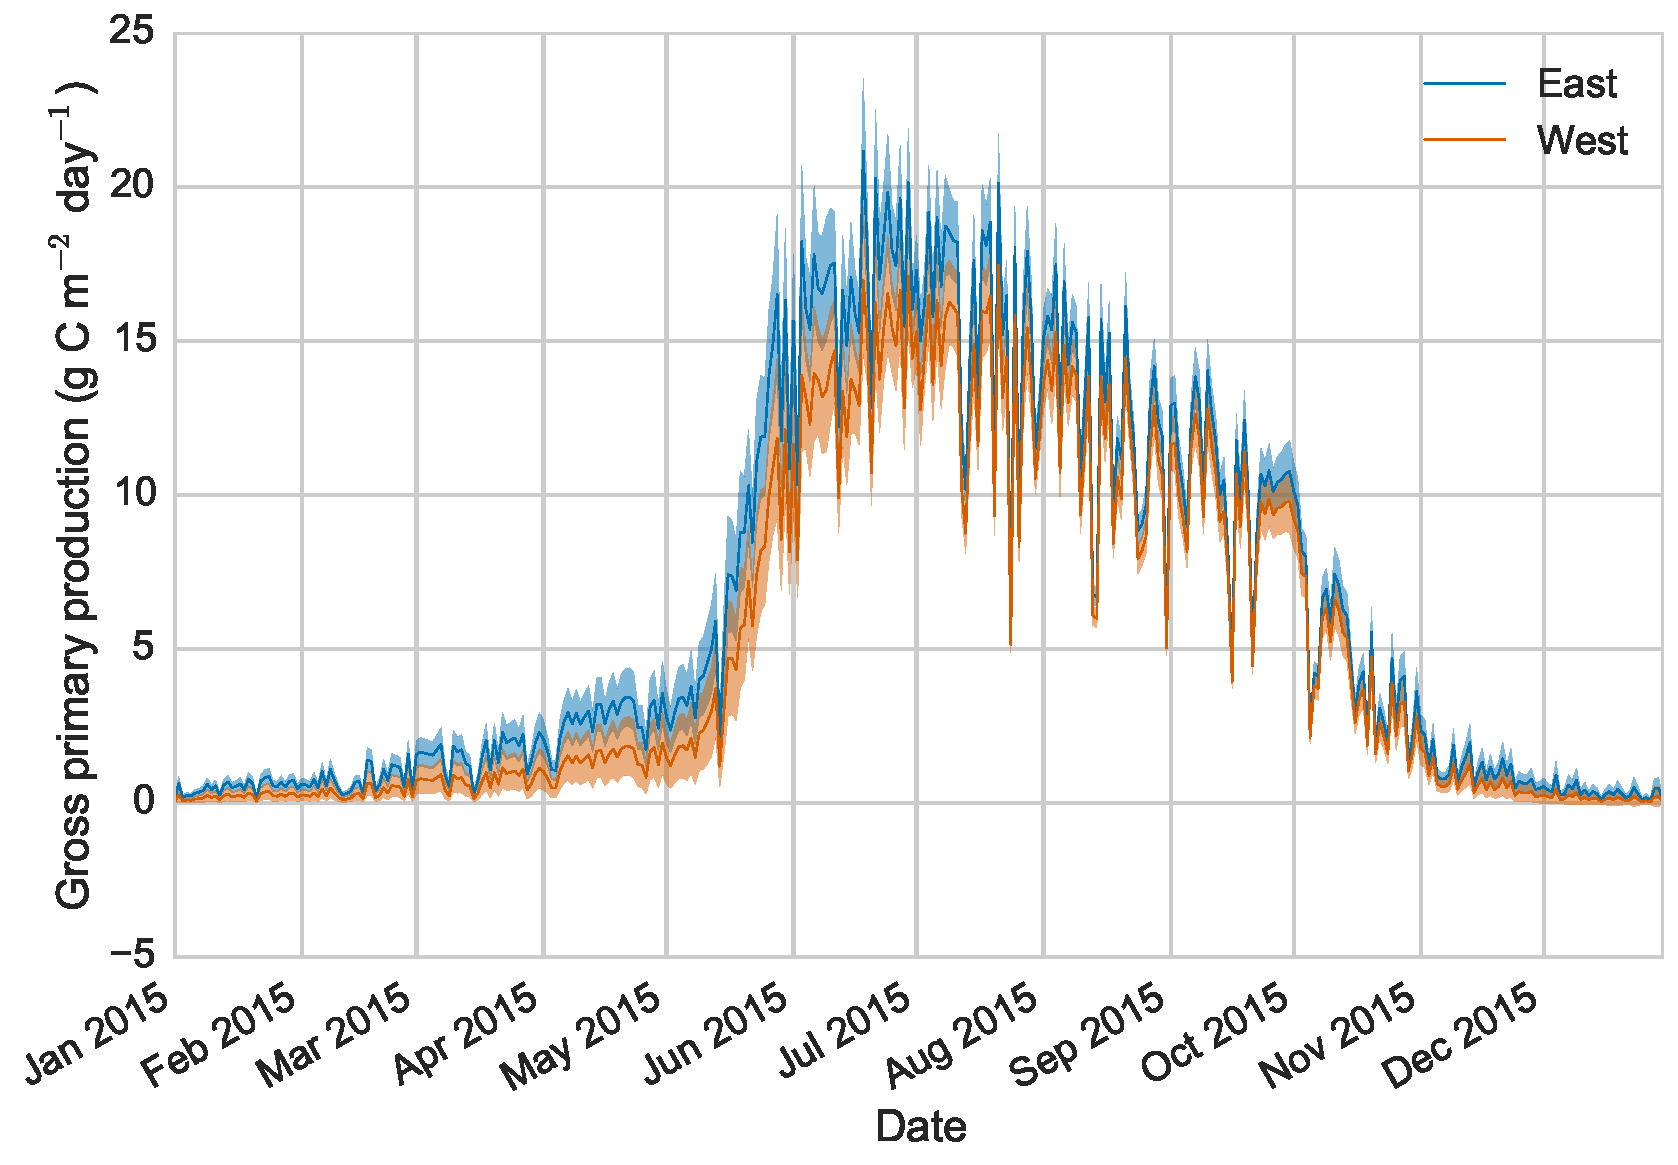
\includegraphics[width=\textwidth]{gpp.pdf}
        \caption{GPP}
        \label{fig:gpp}
        \end{subfigure}
     \begin{subfigure}[b]{0.49\textwidth}
        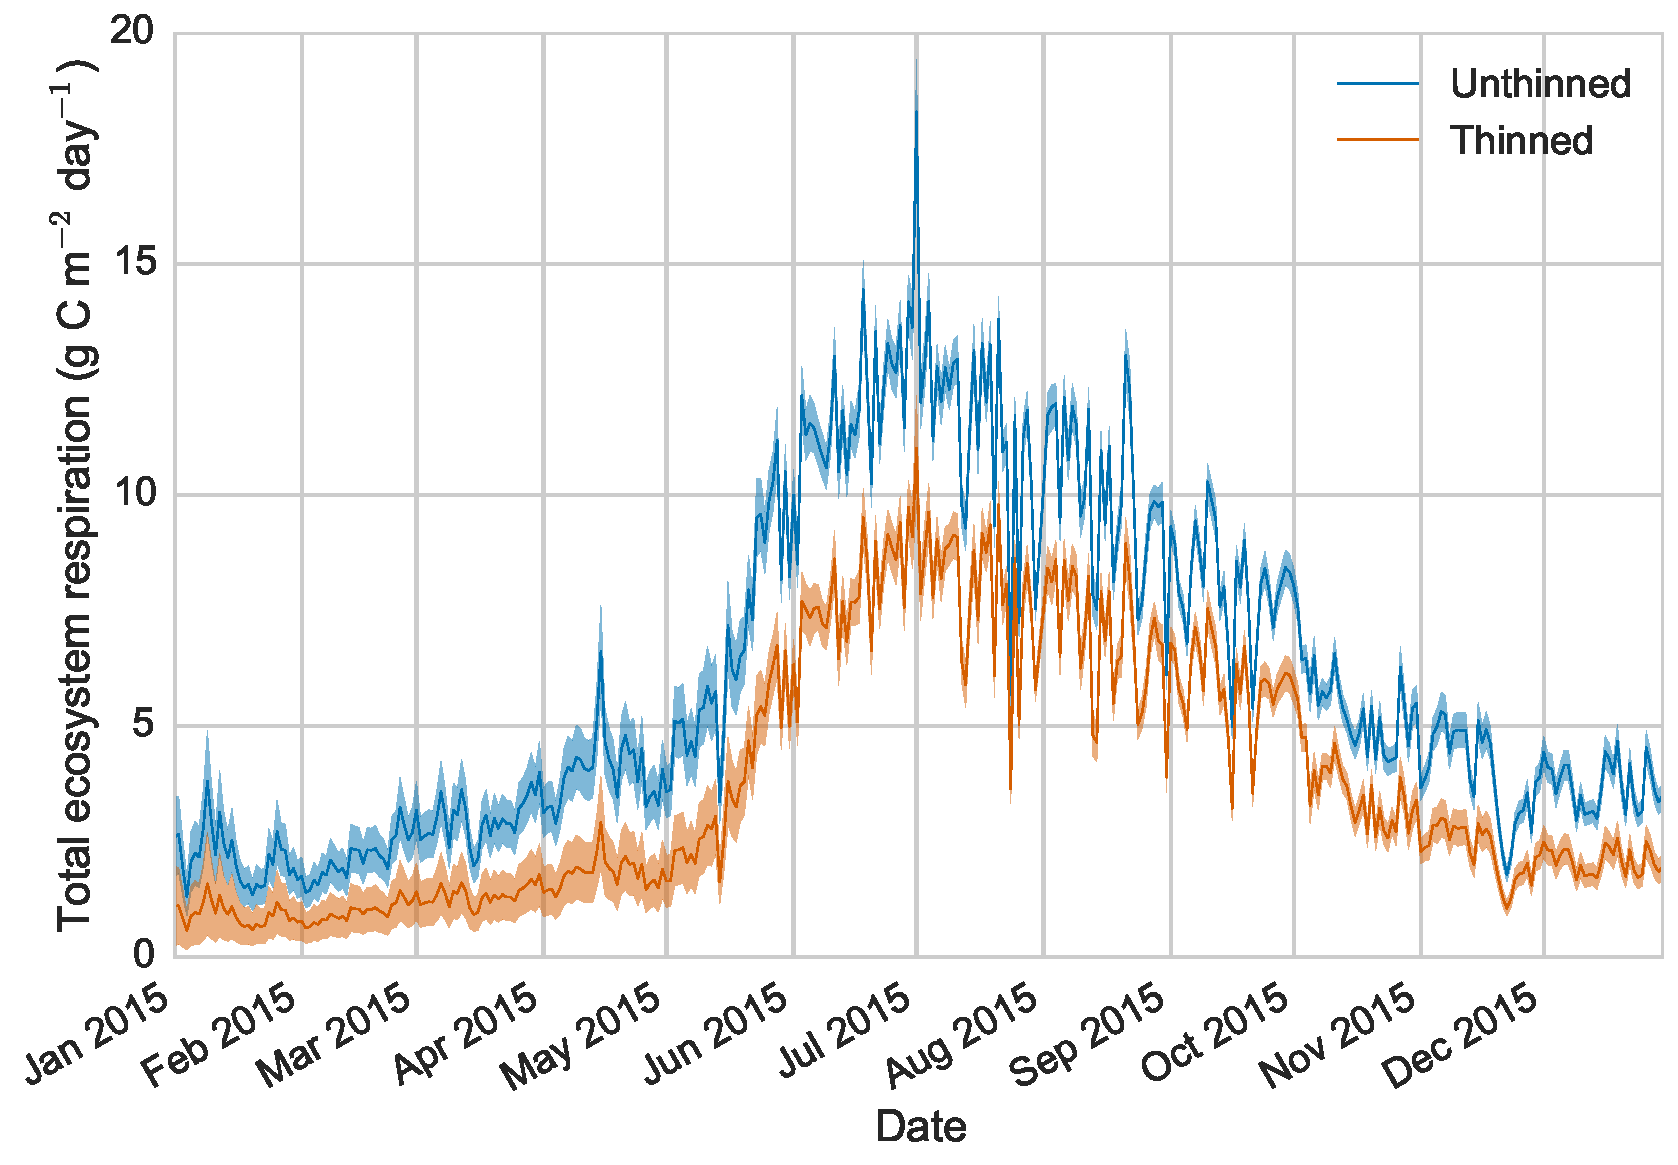
\includegraphics[width=\textwidth]{rt.pdf}
        \caption{Total ecosystem respiration}
        \label{fig:rt}
    \end{subfigure}
    \begin{subfigure}[b]{0.49\textwidth}
        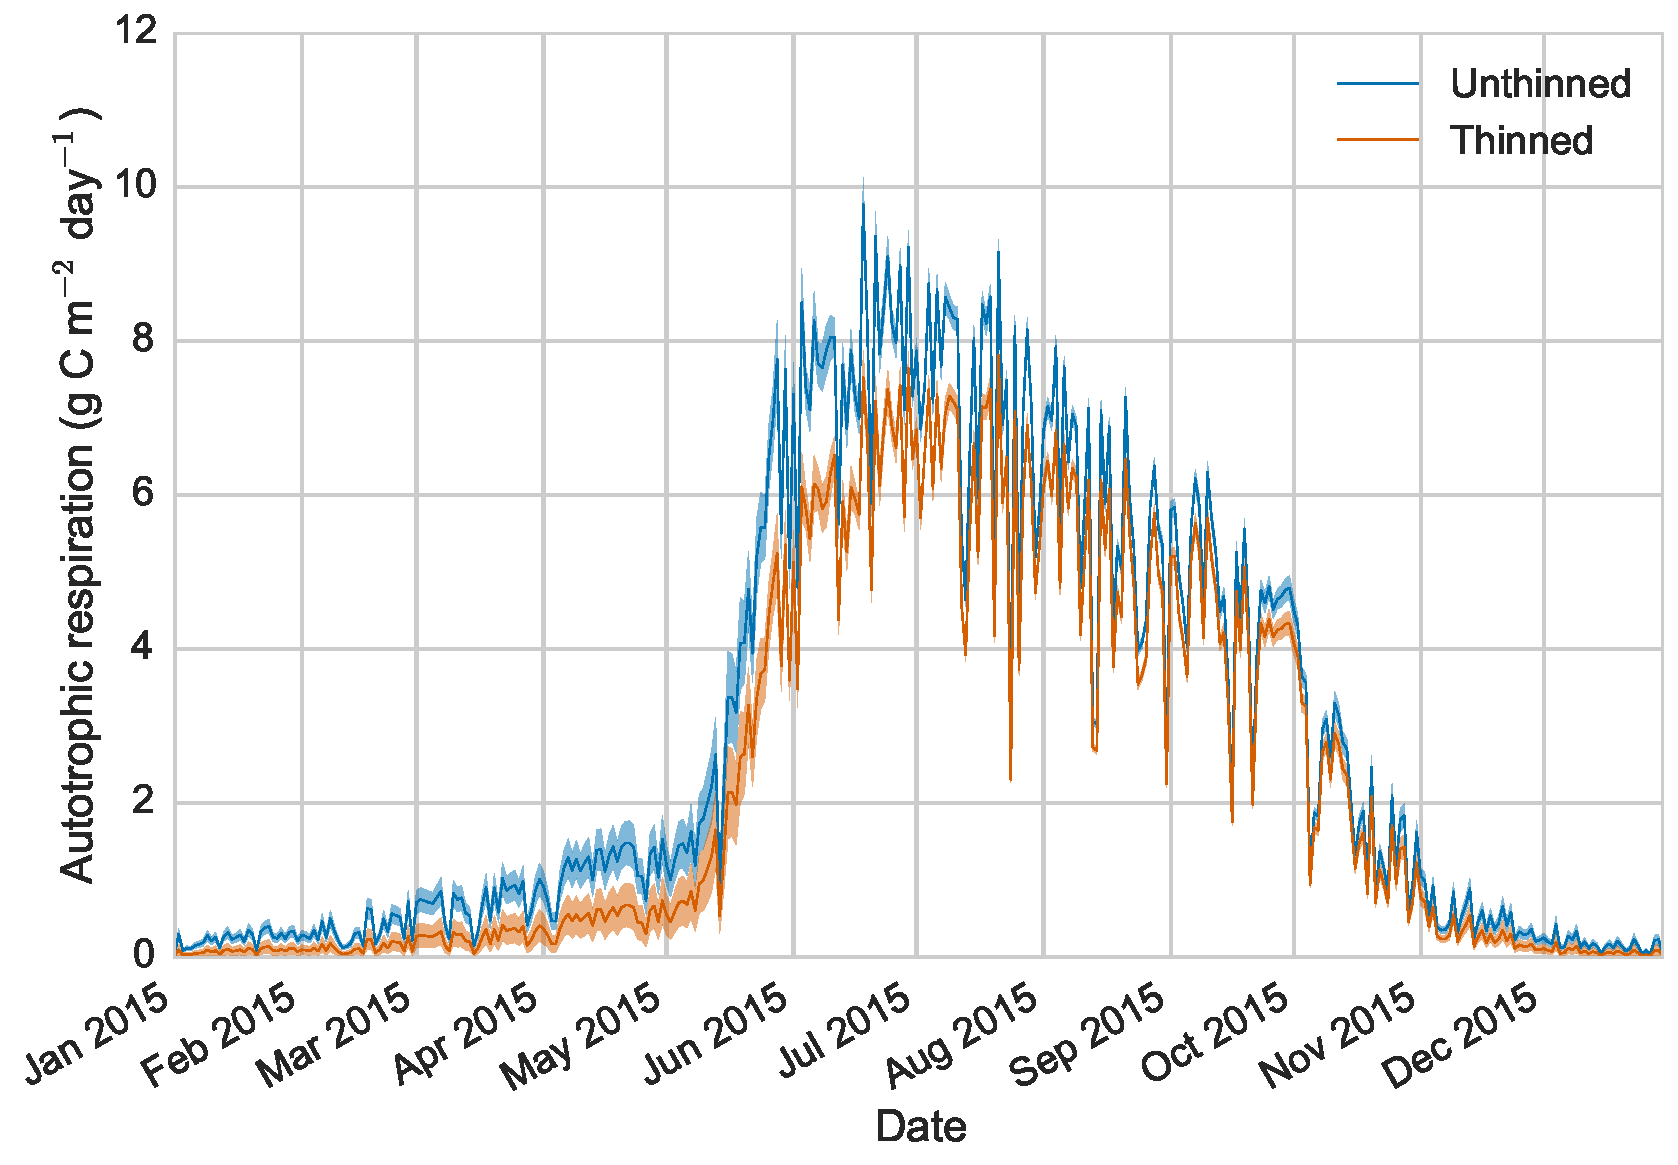
\includegraphics[width=\textwidth]{ra.pdf}
        \caption{Autotrophic respiration}
        \label{fig:ra}
    \end{subfigure}
    \begin{subfigure}[b]{0.49\textwidth}
        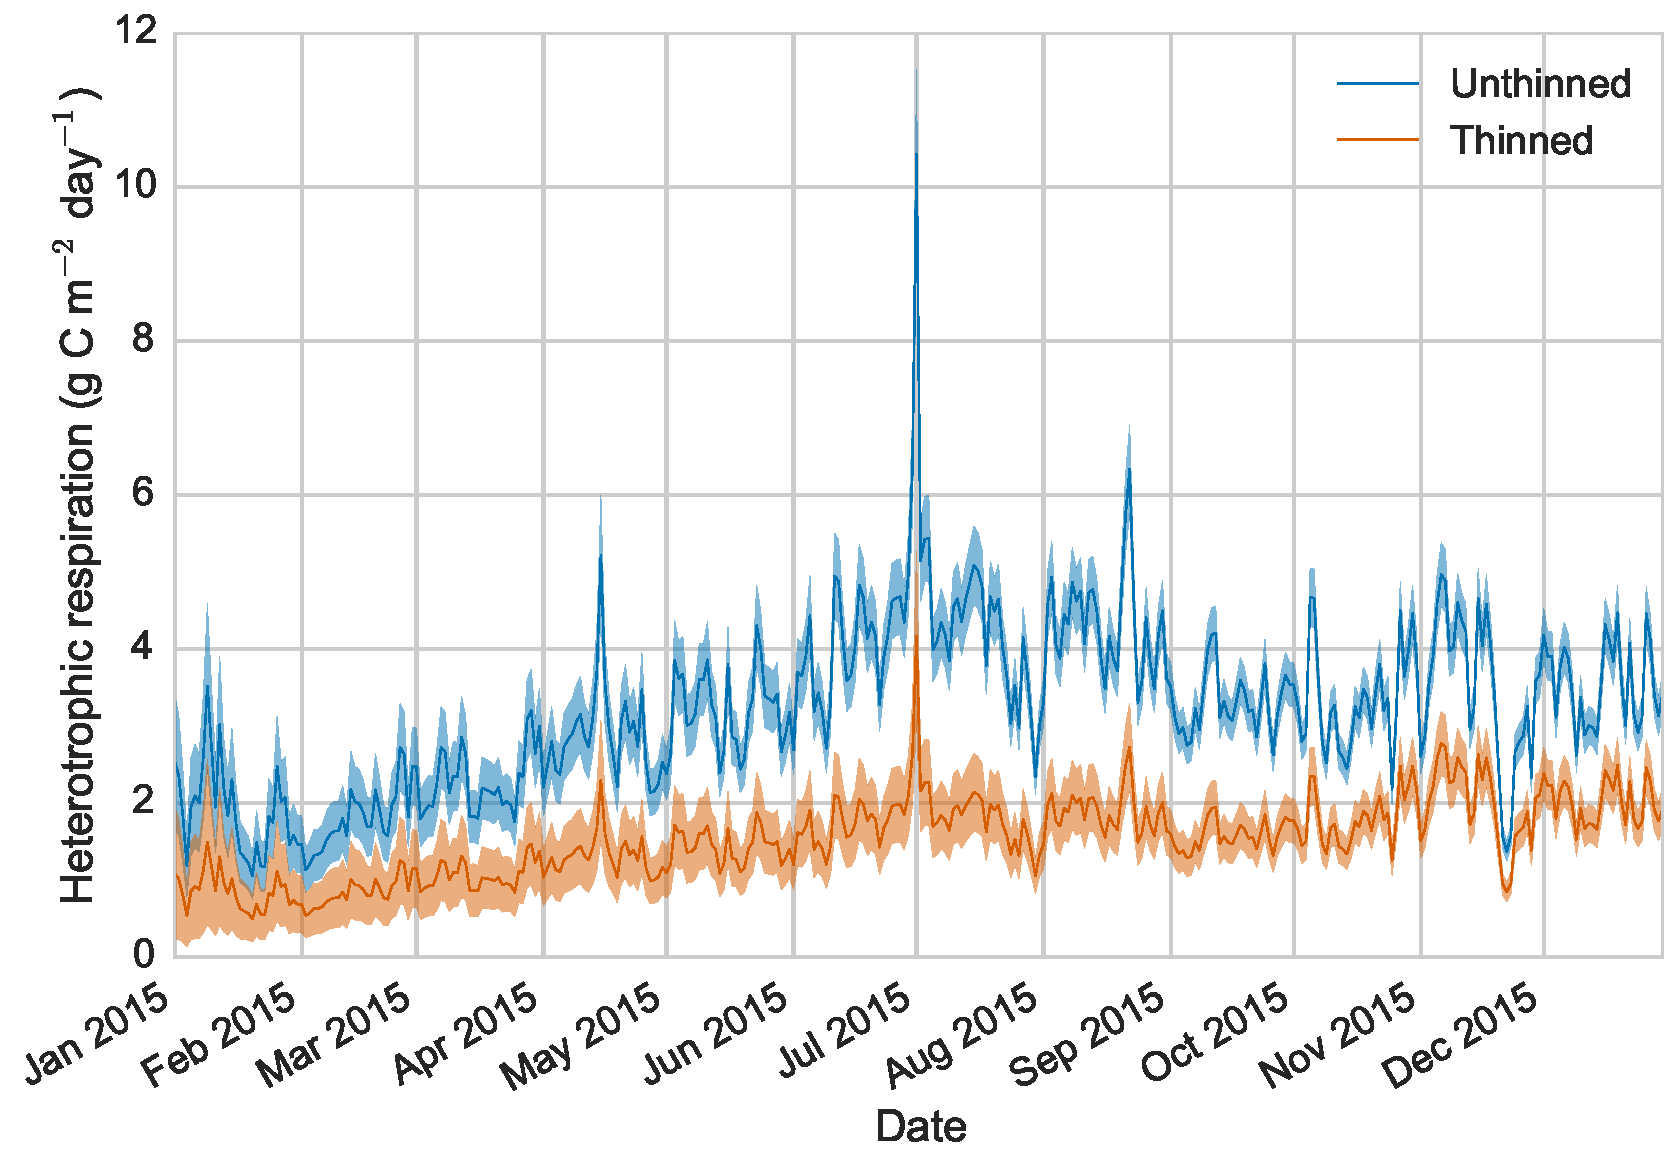
\includegraphics[width=\textwidth]{rh.pdf}
        \caption{Heterotrophic respiration}
        \label{fig:rh}
    \end{subfigure}
    \caption{2015 East and West model trajectories after assimilation. Blue line: model trajectory after assimilation of East data, blue shading: error in model after assimilation (\(\pm\) 1 standard deviation), blue dots: East observations with error bars, orange line: model trajectory after assimilation of West data, orange shading: error in model after assimilation (\(\pm\) 1 standard deviation), orange dots: West observations with error bars.} \label{fig:nee_day}
\end{figure}

\begin{figure}[ht]
    \centering
    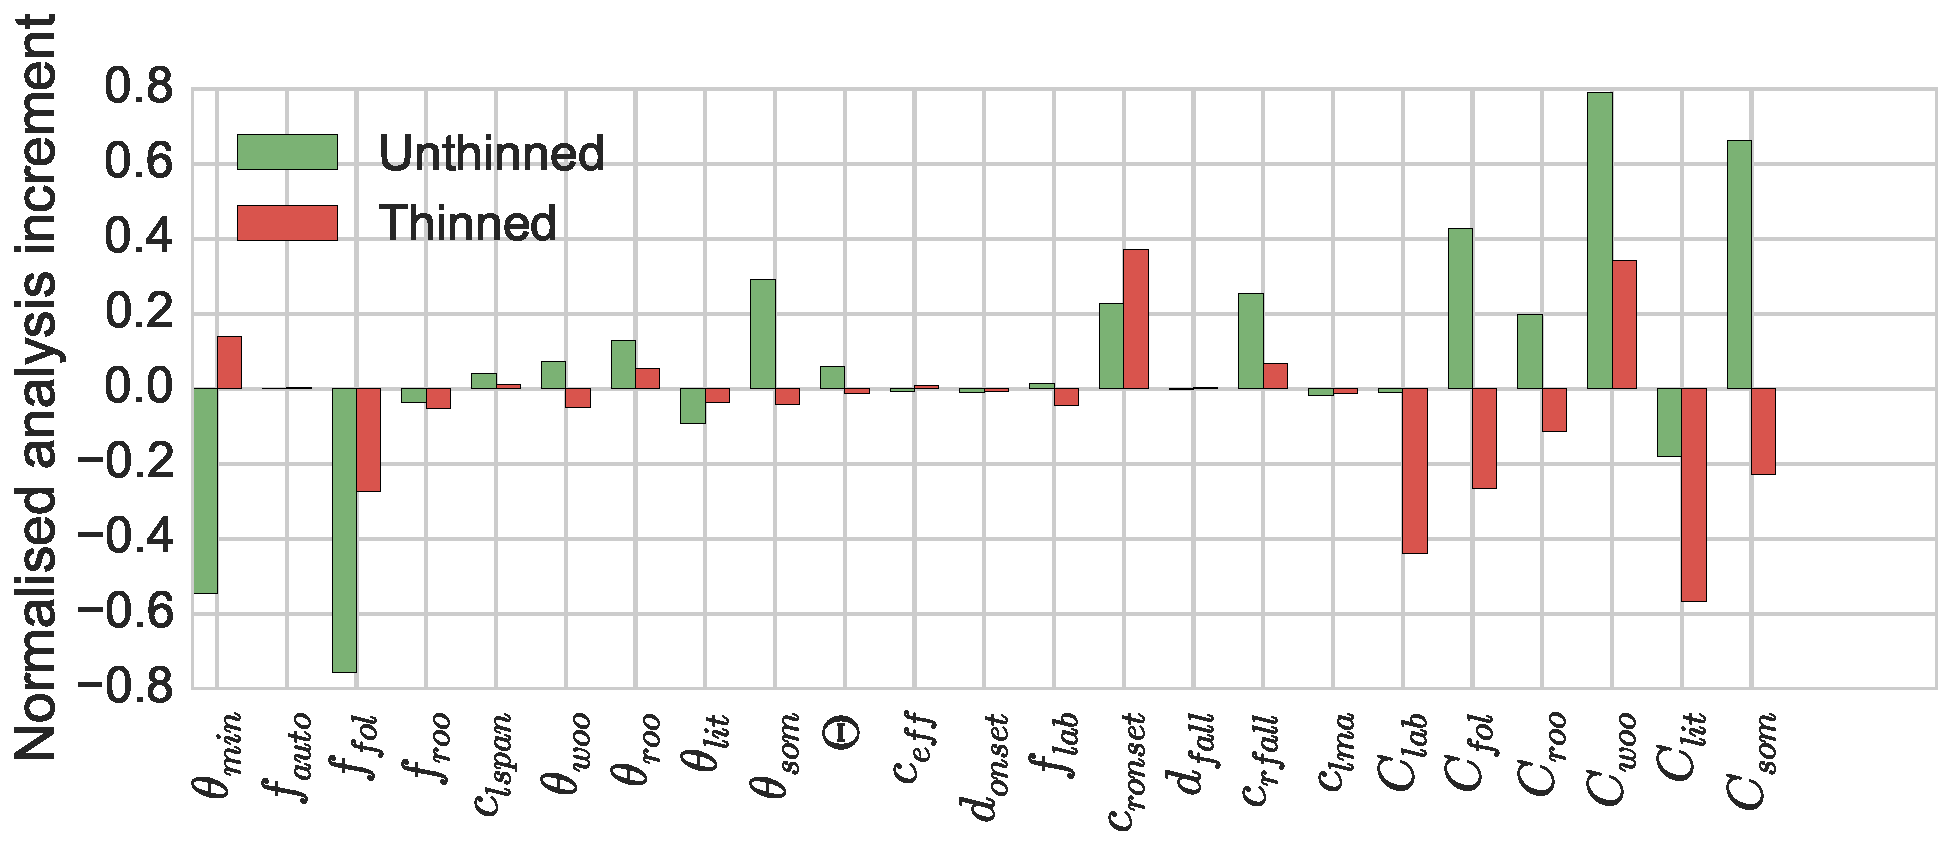
\includegraphics[width=0.8\textwidth]{xa_inc.pdf}
    \caption{Normalised analysis (posterior model) increment \big($\frac{(\textbf{x}^a - \textbf{x}^b)}{\textbf{x}^b}$\big) for the East and West experiments. Explanation of parameter and state variable symbols in table~\ref{table:xbvars}.}
    \label{fig:xa_inc}
\end{figure}

\section{Discussion}
From the assimilation of multiple data streams with a model of ecosystem carbon balance we find evidence that reduced heterotrophic respiration following disturbance allows a managed woodland to exhibit an unchanged net carbon uptake when compared against an undisturbed section of the same woodland. 

\section{Conclusion}
Wrap up the results and discussion.

This supports work suggesting that there could be an upper limit to net carbon uptake of the land surface due to increased GPP leading to increased ecosystem respiration REF Andreas. 

\begin{itemize}
\item We present novel techniques for the assimilation of day/night NEE using a modified observation operator. This facilitates the assimilation of a large amount of data that would have been previously neglected during data processing, without the need to alter the implemented model. Assimilation of NEE at this day/night time step could also help with the partitioning of NEE between GPP and ecosystem respiration.

\item We demonstrate how data assimilation can be used to understand the effect of sudden changes to a studied system. Assimilating all available data streams after an event of disturbance allows us to assess changes to model parameter and state variables due to this disturbance.

\item We find no significant change in net carbon uptake after disturbance for the managed side of the forest, despite a large proportion of trees being lost to felling. This was also found to be true when a similar event occurred in 2007 REF Matt. It would be logical to assume that we would see decreased net carbon uptake due to this disturbance, resulting from fewer trees doing less GPP and heterotrophic respiration continuing at a similar rate as pre-disturbance. From our optimised model we find this unchanged net carbon uptake to be due to reduced heterotrophic respiration. So that even for a demonstrated decrease in GPP we have a relatively unchanged net carbon uptake. This supports work suggesting that there could be an upper limit to net carbon uptake of the land surface due to increased GPP leading to increased ecosystem respiration REF Andreas and others. 



\end{itemize}

\bibliography{../PhD}{}

\section*{Appendix}

\section{DALEC2 equations} \label{sec:dalec_eqns}

The model equations for the carbon pools at day $i$ are as follows:

\begin{align}
GPP^{i} &= ACM(C_{fol}^{i-1}, c_{lma}, c_{eff}, \Psi) \label{GPP}
\\C_{lab}^{i}&=C_{lab}^{i-1}+(1-f_{auto})(1-f_{fol})f_{lab}GPP^{i}-\Phi _{on}C_{lab}^{i-1}, \label{daleclab}
\\C_{fol}^{i}&=C_{fol}^{i-1}+\Phi_{on}C_{lab}^{i-1}+(1-f_{auto})f_{fol}GPP^{i}-\Phi_{off}C_{fol}^{i-1}, \label{dalec1}
\\C_{roo}^{i}&=C_{roo}^{i-1}+(1-f_{auto})(1-f_{fol})(1-f_{lab})f_{roo}GPP^{i}-\theta_{roo}C_{roo}^{i-1}, 
\\C_{woo}^{i}&=C_{woo}^{i-1}+(1-f_{auto})(1-f_{fol})(1-f_{lab})(1-f_{roo})GPP^{i}-\theta_{woo}C_{woo}^{i-1}, 
\\C_{lit}^{i}&=C_{lit}^{i-1}+\theta_{roo}C_{roo}^{i-1}+\Phi_{off}C_{fol}^{i-1}-(\theta_{lit}+\theta_{min})e^{\Theta T^{i-1}}C_{lit}^{i-1}, 
\\C_{som}^{i}&=C_{som}^{i-1}+\theta_{woo}C_{woo}^{i-1}+\theta_{min}e^{\Theta T^{i-1}}C_{lit}^{i-1}-\theta_{som}e^{\Theta T^{i-1}}C_{som}^{i-1}, \label{dalec5}
\end{align}
where $T^{i-1}$ is the daily mean temperature, $\Psi$ represents the meteorological driving data used in the $GPP$ function and $\Phi_{on} / \Phi_{off}$ are functions controlling leaf-on and leaf-off. Descriptions for each model parameter used in equations \eqref{GPP} to \eqref{dalec5} are included in table~\ref{table:xbvars}. DALEC2 can be parameterised for both deciduous and evergreen sites with $\Phi_{on}$ and $\Phi_{off}$ being able to reproduce the phenology of either type of site. The full details of this version of DALEC can be found in \cite{Bloom2015}. 

\begin{table}[ht] 
\begin{center}
	\begin{tabularx}{\textwidth}{| l | X | l | l | l |}
	\hline
	Parameter & Description & \pbox{7cm}{Background\\ vector ($\textbf{x}^{b}$)} & \pbox{7cm}{Standard \\deviation} & Range \\ \hline
$\theta_{min}$ & Litter mineralisation rate (day$^{-1}$) & $9.810\times 10^{-4}$ & $2.030\times 10^{-3}$ & $10^{-5} - 10^{-2}$ \\ \hline
$f_{auto}$ & Autotrophic respiration fraction & $5.190\times 10^{-1}$ & $1.168\times 10^{-1}$ & $0.3 - 0.7$  \\ \hline
$f_{fol}$ & Fraction of GPP allocated to foliage & $1.086\times 10^{-1}$ & $1.116\times 10^{-1}$ & $0.01-0.5$ \\ \hline
$f_{roo}$ & Fraction of GPP allocated to fine roots & $4.844\times 10^{-1}$ & $2.989\times 10^{-1}$ & $0.01-0.5$ \\ \hline
$c_{lspan}$ & Determines annual leaf loss fraction & $1.200\times 10^{0} $ & $1.161\times 10^{-1}$ & $1.0001 - 10$ \\ \hline
$\theta_{woo}$ & Woody carbon turnover rate (day$^{-1}$) & $1.013\times 10^{-4}$ & $1.365\times 10^{-4}$ & $2.5\times10^{-5} - 10^{-3}$ \\ \hline
$\theta_{roo}$ & Fine root carbon turnover rate (day$^{-1}$) & $3.225\times 10^{-3}$ & $2.930\times 10^{-3}$ & $10^{-4} - 10^{-2}$ \\ \hline
$\theta_{lit}$ & Litter carbon turnover rate (day$^{-1}$) & $3.442\times 10^{-3}$ & $3.117\times 10^{-3}$ & $10^{-4} - 10^{-2}$ \\ \hline
$\theta_{som}$ & Soil and organic carbon turnover rate (day$^{-1}$) & $1.113\times 10^{-4}$ & $1.181\times 10^{-4}$ & $10^{-7} - 10^{-3}$ \\ \hline
$\Theta$ & Temperature dependance exponent factor & $4.147\times 10^{-2}$ & $1.623\times 10^{-2}$ & $0.018 - 0.08$ \\ \hline
$c_{eff}$ & Canopy efficiency parameter & $7.144\times 10^{1}$ & $2.042\times 10^{1}$ & $10 - 100$ \\ \hline
$d_{onset}$ & Leaf onset day (day) & $1.158\times 10^{2}$ & $6.257\times 10^{0}$ & $1 - 365$ \\ \hline
$f_{lab}$ & Fraction of GPP allocated to labile carbon pool & $3.204\times 10^{-1}$ & $1.145\times 10^{-1}$ & $0.01 - 0.5$ \\ \hline
$c_{ronset}$ & Labile carbon release period (days) & $4.134\times 10^{1}$ & $1.405\times 10^{1}$ & $10 - 100$ \\ \hline
$d_{fall}$ & Leaf fall day (day) & $2.205\times 10^{2}$ & $3.724\times 10^{1}$ & $1 - 365$ \\ \hline
$c_{rfall}$ & Leaf-fall period (days) & $1.168\times 10^{2}$ & $2.259\times 10^{1}$ & $10 - 100$ \\ \hline
$c_{lma}$ & Leaf mass per area ($\text{g C m}^{-2}$) & $1.285\times 10^{2}$ & $6.410\times 10^{1}$ & $10 - 400$ \\ \hline
$C_{lab}$ & Labile carbon pool ($\text{g C m}^{-2}$) & $1.365\times 10^{2}$ & $6.626\times 10^{1}$ & $10 - 1000$ \\ \hline
$C_{fol}$ & Foliar carbon pool ($\text{g C m}^{-2}$) & $6.864\times 10^{1}$ & $3.590\times 10^{1}$ & $10 - 1000$ \\ \hline
$C_{roo}$ & Fine root carbon pool ($\text{g C m}^{-2}$) & $2.838\times 10^{2}$ & $2.193\times 10^{2}$ & $10 - 1000$ \\ \hline
$C_{woo}$ & Above and below ground woody carbon pool ($\text{gCm}^{-2}$) & $6.506\times 10^{3}$ & $7.143\times 10^{3}$ & $100 - 10^{5}$ \\ \hline
$C_{lit}$ & Litter carbon pool ($\text{g C m}^{-2}$) & $5.988\times 10^{2}$ & $5.450\times 10^{2}$ & $10 - 1000$ \\ \hline
$C_{som}$ & Soil and organic carbon pool ($\text{g C m}^{-2}$) & $1.936\times 10^{3}$ & $1.276\times 10^{3}$ & $100 - 2 \times 10^{5}$  \\ \hline
	\end{tabularx}
	\caption{Parameter values and standard deviations for background vector used in experiments.}
	\label{table:xbvars}
\end{center} 
\end{table}

\end{document}